%\documentclass[a4paper]{report}
\documentclass[a4paper, 12pt, titlepage]{article}

%% Language and font encodings
\usepackage[french]{babel}
\usepackage[utf8]{inputenc}
\usepackage[T1]{fontenc}
\usepackage{microtype}

%% Sets page size and margins
\usepackage[a4paper,top=3cm,bottom=2cm,left=3cm,right=3cm,marginparwidth=1.75cm]{geometry}

%% Useful packages
\usepackage{amsmath}
\usepackage{graphicx}
\usepackage{hyperref}
\hypersetup{%
	colorlinks=true, 	      	% false: boxed links; true: colored links
	linkcolor=black,          	% color of internal links
	urlcolor=blue,           	% color of external links
	citecolor=grey
}
\usepackage{lmodern}
%% ajouter fonte petite capitale grasse à lmodern avec celle de computer modern %%
\rmfamily
\DeclareFontShape{T1}{lmr}{b}{sc}{<->ssub*cmr/bx/sc}{}
\DeclareFontShape{T1}{lmr}{bx}{sc}{<->ssub*cmr/bx/sc}{}
\usepackage{url}
\usepackage[usenames, dvipsnames]{xcolor} % couleurs (nombre de base étendu)

\usepackage{minted}% insérer code source
\definecolor{bg}{rgb}{0.95,0.95,0.95}
\setminted{linenos,bgcolor=bg,tabsize=4,breaklines}

\usepackage{amsmath}
\usepackage{amsfonts}
\usepackage{amssymb}
\usepackage{amsthm}
\usepackage{multicol}
\definecolor{grey}{rgb}{0.96,0.96,0.96}
\definecolor{grey2}{rgb}{0.3,0.3,0.3}

\begin{document}

\title{Book Initiation --- V1}
\author{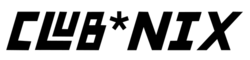
\includegraphics{clubnix}}

\date{\url{https://clubnix.fr}}%}

\maketitle

\tableofcontents

\newpage
~
\newpage

\section{Linux}
 \subsection{GNU-Linux}
    \subsubsection{UNIX}

\paragraph{} \textbf{UNIX} est un \textbf{systeme d'exploitation} multi-tâches
et multi- utilisateurs créé en \textbf{1969}. Il est composé de plusieurs
composants:

\begin{description}
	\item[Le noyau:] aussi appelé ``kernel'' en anglais. C'est un logiciel
		central au système d'exploitation; il fait le lien entre le matériel et
		les logiciels plus normaux.
	\item[Un environnement de développement:] ou tout simplement des outils qui
		permettent de créer de nouveaux logiciels/outils.
	\item[Des commandes] qui permettent d'exécuter des actions qu'on attend
		d'un système d'exploitation, comme manipuler les fichiers, aller sur
		internet, etc.
	\item[De la documentation] qui explique le fonctionnement du système et des
		outils fournis.
\end{description}

\paragraph{} C'est une \textbf{marque deposée de l'OpenGroup}. Son nom est un
dérivé de "Unics" (\textit{Uniplexed Information and Computing Service}). C'est
un jeu de mot avec "Multics" (un autre système) qui vise à offrir simultanément
plusieurs services à un ensemble d'utilisateurs.

UNIX a donné naissance à une \textbf{famille de systèmes} comme BSD, GNU/Linux,
iOS ou encore MacOS, eux-mêmes divisés en variantes de systèmes d'exploitation
aux \textbf{normes POSIX}. Cette norme technique standardise des outils ou des
fonctionnements que l'on devrait retrouver dans un système d'exploitation.

\paragraph{} Il faut savoir que la quasi-totalité des systèmes PC ou mobiles (à
l'exception des systèmes Windows) sont sur des systèmes basés sur la norme POSIX (y compris
ceux de la marque Apple). D'une certaine manière, on peut dire qu'ils sont
descendants ou directement reliés à UNIX.

\subsubsection{GNU: "GNU's Not UNIX"}\label{subsubsec:gnu}

\paragraph{} GNU est un \textbf{projet des années 1990} lancé par Richard
Stallman. C'est un \textbf{système d'exploitation libre}, bien qu'incomplet,
compatible avec la norme POSIX. GNU est incomplet car il lui manque un noyau
viable; il est donc très souvent utilisé avec le noyau Linux, développé par
Linus Torvalds, ce qui a donné le projet GNU/Linux (c.f. section
\ref{subsubsec:gnulinux}).

Sa \textbf{philosophie} est de maintenir intacts les \textbf{tradictions hackers
de partage} dans un monde de plus en plus marqué par l'empreinte du droit
d'auteur. Il se bat donc pour une \textbf{libre diffusion des connaissances}.
"GNU vise à ne laisser l'homme devenir ni l'esclave de la machine ni de ceux
qui auraient l'exclusivité de sa programmation".

\paragraph{} Il est \textbf{utilisable et partageable librement par tous},
ainsi chacun complète petit a petit l'architecture initiale de GNU pour le
rendre meilleur. C'est dans ce contexte que le projet invite la communauté de
hackers à le rejoindre et à participer à son développement. Il faut savoir
qu'il est composé :

\begin{itemize}
	\item d'un éditeur de texte (emacs),
	\item d'un compilateur très performant (gcc),
	\item d'un débogueur (gdb),
	\item d'un langage de script (bash),
	\item de bibliothèques de systèmes (glibc),
\end{itemize}

\subsubsection{GNU/Linux}\label{subsubsec:gnulinux}

\paragraph{} GNU/Linux a été créé en \textbf{1991}. Il est \textbf{initié par
le projet Debian} et la naissance du noyau Linux. Il crédite donc à la fois
Linux et GNU \textit{mais l'usage de Linux est plus connu au grand public}.

Il est alors toujours basé sur le \textbf{mouvement du logiciel libre et du
mode opératoire du hacker}. Cette association a eu lieu pour combler le vide
causé par le développement inachevé de GNU (c.f. section \ref{subsubsec:gnu}).

\paragraph{} Il est utilisé sur la plupart des téléphones portables (par
exemple Android) comme sur les super-ordinateurs. Ce projet eut un grand impact
dans le monde des serveurs informatiques. GNU/Linux veut casser le fait qu'à
l'origine il fallait des connaissances solides en informatique pour utiliser un
système d'exploitation (\textit{pas d'interface graphique et besoin d'installer
toutes les applications soi-même}).

Il a donc été un important vecteur de \textbf{popularisation du mouvement de
l'open source}. Il a eu des \textbf{centaines de milliers de redistributions}
avec des versions différentes pour plaire à tous les goûts (en fonction des
besoins, configurations, sécurité, ...\textit{voir différents OS}). GNU/Linux a
remplacé d'autres systèmes de type UNIX et/ou évite l'achat d'une licence
Windows (qui est très chère à l'achat).

\paragraph{} Aujourd'hui on peut retrouver tous les équivalents des
logiciels/applications qu'il y a sous Windows mais en Open Source.

 \subsection{Différents OS}
    En informatique, un systeme d'exploitation est un ensemble de programmes qui dirige l'utilisation des capacites d'un ordinateur par des logiciels applicatifs.\newline


\subsection{Differents OS}
\begin{itemize}
\item MacOS (series d'interfaces graphiques basé sur l'operation des systemes developé par Apple pour leur Macintosh),
\item iOS (systeme d'operation pour mobile developper et distribuer par Apple pour iPhone et iPod),
\item \textbf{Linux} (c'est un Unix. systeme d'operation pour ordinateur assembler sous le modele du "free and open source software"),
\item Android (c'est un derivé de Linux. systeme d'operation designer pricipalement pour les mobiles tactiles comme les smartphones et les tablettes, initialement developper par Android),
\item Microsoft Windows (serie d'interface graphique developper et commercialiser par Microsft),
\item BSD/OS (reputaté pour reabiliter le role des serveurs, oganiser par les programmeur d'Unix, utiliser pour une utilisateur personnel du web).\newline
\end{itemize}


\subsection{differentes familles d'OS Linux} 

\begin{itemize}
\item \textbf{Debian/Ubuntu} : \textit{1993}
    \begin{itemize}
    \item developpé par SPI (\textit{Software in the Public Interest}),
	\item caractere non commercial et mode de gouvernance cooperatif,
	\item deja installer avec son noyau, ses pilotes, son programme d'installation de distribution, ses logiciels "utiles" (pour le WiFi, une navigateur web, ...) ,
	\item reuni une dizaine de sous-famille Debian avec le même noyau mais avec une architecture differente, dont les plus connus sont : KaliLinux, Kubunto, Raspbian, Ubuntu, Xubunto.\newline 
    \end{itemize}
   
\item \textbf{Red Hat/Cent OS/Fedora} : \textit{1994}
    \begin{itemize}
	\item developper et distribuer par l'entreprise Red Hat (entreprise dedier aux logiciels Open sources + distributeur de systeme d'exploitation Linux),
	\item plusieurs grosse distribution son issus de ce dev : Fedora, Enigma, ...
	\item principalement destinee aux serveurs des entreprises,
	\item voulait faire passer doucement les utilisateurs Windows sous Linux.\newline
	\end{itemize}

\item \textbf{Arch} : \textit{2002}
    \begin{itemize}
	\item accent sur la simplicité et legerete : parfait pour les utilisateurs avancés,
	\item pas d'outils graphiques : pour resoudre tout les problemes du systemes,
	\item contribution ouverte (OpenSource) tant que cela respecte sa philosophie.\newline
	\end{itemize}
	
\item \textbf{Suse/OpenSuse} : \textit{1994}
    \begin{itemize}
	\item distribution communautaire et commerciale,
	\item destine a l'utilisation en entreprise mais toujours en Open-Source,
	\item cycle de developpement long mais cycle de vie long,
	\item disponible par la vente (licence et mise a jour).
	\end{itemize}
\end{itemize}


\newpage
\section{Ecrire un document texte}
  \subsection{LaTeX}
    \subsubsection{Histoire et Principe}

\LaTeX  a été créé en 1983, c'est un \textbf{langage et un système de composition de documents}.
Il sert principalement à de la mise en page simple de documents et a pour but de
 séparer le fond et la forme.

\LaTeX  est devenu le langage privilégié pour les documents scientifiques du fait
 de sa simplicité.\newline

Pour rédiger du \LaTeX , il faut uniquement se concentrer sur la structure
logique du document et son contenu car le logiciel s'occupe de la mise en page
automatiquement.
Vous pouvez écrire en \LaTeX  grâce à différents logiciels d’éditeurs de texte
dédiés comme TexMaker, Texlive, TeXworks, TexMacs, ...
Dans ces éditeurs, il est possible de voir directement la mise en page en format
PDF lorsqu'il est compilé.
Mais il est également possible de manipuler \LaTeX  simplement à partir d'un
terminal ou de gedit par exemple.\newline

L'évolution de \LaTeX  est assurée par la communauté d'utilisateurs qui regroupe
des étudiants et des professeurs de mathématiques ou de physique, comme des
musiciens et ingénieurs en informatique notamment.


\subsubsection{Différences avec Word}

Il faut d'abord savoir que les deux logiciels ne se comportent et ne s'utilisent pas de la même façon.

\begin{itemize}
\item La mise en page (images, figures, légendes, formules mathématiques, dessins, tableaux, ...) sur Word est une rude manipulation
 qui fait perdre du temps. \LaTeX  le fait tout seul, mais son interface austère fait "peur" aux débutants.
  Pourtant il suffit de lui dire quel type de documents on souhaite obtenir pour obtenir quelque chose de lisible
  et adapté avec les normes éditoriales ;
\item \LaTeX  est gratuit (et même libre), contrairement à Word ;
\item Les formules mathématiques sont simples d'écriture sur \LaTeX  ;
\item Tout est modifiable et paramétrable avec \LaTeX  à n'importe quel moment
(\textit{si au bout de la 100 ème page vous vous rendez compte que vous voulez
changer de police, uniquement sur tous les titres par exemple}) ;
\item La gestion de documents longs est intuitive sur \LaTeX , contrairement à
la complexité sur Word lorsqu'il faut gérer
la mise en page identique ;
\item \LaTeX  peut générer automatiquement des bibliothèques ou tables de matières beaucoup plus facilement que sur Word ;
\item Accéder à la création des PDF rapidement sur \LaTeX  ;
\end{itemize}


\subsubsection{Utilisation}

Le système de balisage est assez semblable au langage HTML. Il est donc possible
de \textbf{créer ou modifier des macro-commandes} afin d'ajouter des raccourcis.
\textit{Par exemple pour regrouper plusieurs instructions en une seule.}
Comme ce langage a été créé avant le Unicode, tous les caractères peuvent
s'écrire en ASCII (mais ce n'est plus nécessaire).

Il faut tout d'abord configuration les packages à utiliser pour déterminer la
langue d’écriture, les marges, polices d’écriture, couleur et taille de
l’écriture, style du document, etc ...
Tous ces packages \textbf{peuvent être trouvés documentés sur Internet}, vous
pouvez donc simplement les importer.\newline

Voici les principales instructions qui vous serviront :

\begin{itemize}
\item Partie : $ \setminus part\lbrace \textit{nom\_ de\_ la\_ partie} \rbrace $

\item Section : $ \setminus section\lbrace \textit{nom\_ de\_ la\_ partie}\rbrace $

\item Sous-section : $ \setminus subsection\lbrace \textit{nom\_ de\_ la\_ partie} \rbrace $

\item Paragraphe : $ \setminus paragraph\lbrace \textit{nom\_ de\_ la\_ partie}\rbrace $

\item Saut de ligne : $ \setminus newline ou \setminus \setminus $

\item Liste : $ commencer par \setminus begin \lbrace itemize \rbrace puis pour chaque tiret \setminus item et conclure
par \setminus end\lbrace itemize \rbrace $ \textit{ NB : pour modifier les puces il suffit de mettre la puces souhaitées
entre $ [  ] $ apres $ \setminus item $}
\newline pour des listes numérotées il faut écrire $\setminus begin\lbrace enumerate\rbrace $

\item très très petite écriture : $ \setminus scriptsize $

\item très petite écriture : $ \setminus footnotesize $

\item petite écriture : $ \setminus small $

\item grande écriture : $ \setminus large$

\item très grande écriture : $ \setminus LARGE $

\item très très grande écriture : $ \setminus huge $

\item Gras :  $ \setminus textbf\lbrace\rbrace $
\item Italique :  $ \setminus textit\lbrace\rbrace $
\item Penché :  $ \setminus textsl\lbrace\rbrace $
\item Machine à écrire :  $ \setminus texttt\lbrace\rbrace $
\item Exposant :  $ \setminus textsuperscript\lbrace\rbrace $
\item Encadré :  $ \setminus fbox\lbrace\rbrace $
\item Souligné :  $ \setminus ul\lbrace\rbrace $
\item Barré :  $ \setminus st\lbrace\rbrace $
\end{itemize}

  \subsection{Markdown}
    \subsection{Histoire}

Le markdown est un \textbf{langage de balisage} crée en 2004. Il est facile à manipuler, donc simple à écrire et a lire sans connaître les balises.
Le markdown peut être écrit sur n'importe quel éditeur de texte, il suffit lorsque le document est prêt a être enregistrer de nommer le document puis d'inscrire "\textbf{.md}".

\subsection{Instruction}

Les instructions sont \textbf{très simple et peuvent être combiné}. 
On va voir quelques instructions de bases : 

\subsubsection{Police d'un texte}
\begin{itemize}
	\item Italique : encadrée le(s) mot(s) désiré(s) par * ou _
	\item Gras :  le(s) mot(s) désiré(s) par **
	\item Souligner : encadrée le(s) mot(s) désiré(s) par __
	\item Barré : encadrée le(s) mot(s) désiré(s) par ~~
	\item souligner les titres : mettre sur une ligne en dessous des = ou -
\end{itemize}

\subsubsection{Mise en forme du texte}
\begin{itemize}
	\item commencer un paragraphe : mettre 4 espaces
	\item délimiter un paragraphe : sauter une ligne
	\item retour a la ligne : deux espaces a la fin de phrase
	\item titre : # (rajouter des # par sous niveaux de paragraphes)
\end{itemize}

\subsubsection{Ajout d'élément au texte}
\begin{itemize}
	\item bloc de code : encadrée le(s) mot(s) désiré(s) par ```
	\item citation : commercer par >
	\item liste : commencer par * ou - ou +
	\item liste ordonnée : commencer par 1. 2. 3. ...
	\item cases a cocher : [ ] ou [x]
	\item tableau : 
		- delimité les colonnes par : |
		- delimité les titres des autres lignes par : :-----:
	\item lien : 
		- en hypertexte : l'encadré en < et >
		- en bouton : [ \textit{nom du bouton} ](#){.btn }
	\item mage : ![ \textit{texte} ]( \textit{url de l'image} )
\end{itemize}

\newpage
\section{Terminal}
  \subsection{Terminal}
    \subsubsection{Quoi et pourquoi ?}

\paragraph{} Le terminal est un programme qui permet d'exécuter des commandes
sous forme de texte.

Les commandes permettent en une ligne de texte d'effectuer des
opérations qui peuvent s'avérer très longues avec l'interface graphique. Par
exemple, modifier les droits d'accès ou d'écriture à un fichier s'effectue en
une dizaine de clics avec l'interface graphique, alors que la commande
\texttt{chmod} avec les droits voulus et le nom du fichier le fait
instantanément.

\subsubsection{Ouvrir une console et s'en servir}

\paragraph{} Pour ouvrir une console de terminal, on peut:

\begin{itemize}
	\item chercher terminal dans la barre de recherche;
	\item avec le raccourci clavier disponible sur la plupart des
		environnements de bureau avec Ctrl + Alt + T.
\end{itemize}

Une première ligne apparaît, et est comme ceci:

\begin{itemize}
	\item \mintinline{console}{utilisateur@nom_du_pc:~$}
\end{itemize}

Tapez alors votre ligne de commande puis \textit{Enter} pour l'exécuter.\newline

Il existe de nombreux outils dans le terminal, que nous allons voir ici:

\paragraph{Arrêter une commande} Il est possible de lancer une commande puis de
l'arrêter manuellement sans attendre qu'elle se termine.

Par exemple, vous avez lancé une commande ping pour tester votre réseau. La
commande ping ne s'arrête que si on lui demande. On peut alors l'interrompre
avec le raccourci clavier suivant: \textit{Ctrl + C}. Attention cependant. Même
si sur la commande ping l'arrêt de la commande n'a pas d'impact, ce n'est pas
le cas pour toutes les commandes. \textbf{Ctrl + C est une façon relativement
brutale d'arrêter un programme.}

\paragraph{Copier-coller} Copier-coller une ligne de commande depuis un
terminal est possible, mais pas avec les raccourcis claviers classiques. En
effet, Ctrl + C est déjà un raccourci clavier du terminal. Il faut donc faire
\textit{Ctrl + Shift + C} pour copier une ligne et \textit{Ctrl + Shift + V}
pour coller. Vous pouvez aussi, pour les ordinateurs en disposant, sélectionner
la ligne et cliquer sur le clic du milieu (ou la molette de la souris) afin de
coller la ligne.

Il faut faire attention toutefois avec le copier coller depuis les forums. En
effet, si vous copiez collez une suite de commandes avec des retours à la ligne
comme par exemple:

\begin{itemize}
	\item \textit{ls}
	\item \textit{cd dossier}
	\item \textit{cat fichier}
\end{itemize}

Le terminal exécutera les deux premières commandes car elles sont séparées par
un retour à la ligne. Cela peut être très pratique mais aussi dangereux.

\subsubsection{L'auto-complétion}

Certaines lignes peuvent être longues à taper. Le terminal met à disposition une
touche permettant de compléter la fin de la commande et même parfois les
arguments de la commande. C'est la touche Tab. Après avoir tapé 3 lettres, vous
pouvez demander l'auto-complétion. C'est le cas par exemple pour un nom de
fichier très long ou de paquets. Il suffit alors de taper "cd début + Tab " et
le terminal finira à votre place. Lorsque plusieurs fichiers ont le même début
de nom, le terminal vous les proposera alors en dessous de votre ligne de
commande.

\paragraph{Le manuel} La plupart des commandes disposent d'un manuel, qui
renseigne sur les paramètres de la commande, son utilité, ou encore comment
l'utiliser. Pour ouvrir le manuel d'une commande, on tape dans le terminal
\mintinline{bash}{man 'nom de la commande'}.

\paragraph{Retrouver une commande déjà tapée précédemment} Pour retrouver une
commande déjà tapée, on peut cliquer sur la flèche du haut. Un clic remonte
d'une commande.

De ce fait, si vous souhaitez taper une commande très longue et que vous avez
déjà tapée il y a quelques temps, cliquez sur la flèche du haut autant de fois
que nécessaire pour la retrouver.

\subsubsection{Les droits SUDO}

\paragraph{} Pour exécuter certaines commandes, notamment installer des paquets
ou redémarrer la machine, le terminal a besoin des droits super-utilisateur.
Cela se fait avec la commande SUDO, qui signifie Super Utilisateur DO et qui
permet ``d'élever'' une commande avec les accès super-utilisateur. Quiconque
détient ces droits peut passer des commandes capables de modifier gravement la
machine sans restrictions, donc à utiliser avec précaution.

Pour lancer une commande administrateur système, il faut taper:

\mintinline{bash}{sudo nom_de_la_commande}.

Par exemple pour installer un programme sous Debian/Ubuntu:

\mintinline{bash}{sudo apt install nom_du_programme}.

Le terminal va alors vous demander votre mot de passe administrateur avant de
lancer la commande.

\paragraph{} Si le mot de passe ne s'affiche pas, ni même des astérisques ou
autre, c'est normal: c'est pour renforcer la sécurité car personne ne saura
la taille de ce mot de passe en regardant votre écran. Attention, vous êtes le
seul responsable de votre machine et lancer des commandes sudo sans être sûr de
leur impact pourraient complètement détruire votre machine.

\subsubsection{Les questions des commandes}

\paragraph{} Certaines commandes vous posent des questions, comme par exemple
lors de l'installation d'un paquet ces questions sont de la forme:

\begin{itemize}
	\item ``\texttt{question [Y/N]}''. Il faut alors taper Y (pour yes) ou N
		(pour no) puis entrer afin de répondre à la question.
	\item ``\texttt{question [Y/n]}'' ou ``\texttt{question [y/N]}'' C'est une
		variante dans laquelle vous pouvez toujours taper y ou n
		mais aussi directement entrée. La réponse prise en compte sera celle en
		majuscule.
\end{itemize}

\textit{Il existe un poly regroupant les principales commandes terminal
disponibles sur le GitHub du club.}

  \subsection{Bash}
    \subsubsection{Bash et scripts}

Le bash est un interpréteur de script natif aux systèmes d'exploitation sous
environnement Unix.

\paragraph{A quoi ça sert ?}

Le bash permet l'exécution de scripts, petits morceaux de code, souvent exécutés
 au démarrage, afin d'effectuer une tâche précise.
Par exemple, l'ensemble des applications s'ouvrant au démarrage sont regroupées
 dans un script. Bash permet l'interprétation des commandes shell.
Une commande shell est une chaîne de caractères en minuscules qui peut être
invoquée au travers d'un invite de commande ou d'un script.
 Des options et des arguments peuvent la compléter.

Le bash propose différents traitements des commandes :
\begin{itemize}
  \item Les commandes simultanées : com1 \& com2 \& com3 \& ... \& comN. Les commandes com1 à comN sont exécutées simultanéments;
  \item Les commandes successives : com1 ; com2 ; com3 ; ... ; comN. Les commandes com 1 à comN sont exécutées les unes après les autres;
  \item etc,...\newline
\end{itemize}

Il existe deux modes de fonctionnement du bash :
\begin{itemize}
  \item Le mode interactif : Le terminal fonctionne avec le bash. lorsque l'on
  tape une commande manuellement dans le terminal, on crée en réalité un mini
  script d'une ligne, interprété par bash puis executé;
  \item Le mode batch : bash exécute automatiquement un script contenu dans un
  fichier texte contenant les commandes à utiliser. Ce fichier doit être
  exécutable (réglable avec chmod).
\end{itemize}


\paragraph{L'interprétation d'une ligne de commande}

Chaque interprétation d'une ligne de commande d'un script repose sur des codes bien stricts :
\begin{itemize}
  \item Le premier mot de la ligne est interprété comme le nom de la commande;
  \item Chaque mot est séparé par un ou plusieurs caractères de séparation (espace, tabulation, tiret, underscore ...);
  \item La fin de la ligne se termine par un ';', comme dans la plupart des langages de programmation, ou un retour à la ligne
\end{itemize}


Pour plus d'informations sur les lignes de commandes bash, il existe un poly sur les commandes du terminal disponible sur le GitHub du club.

  \section{SSH}
    \subsubsection{Définition}

SSH signifie "Secure Shell" est un protocole sécurisé pour les communications à distance créé en 1995 par Tatu Ylönen. Pour rappel un Shell va permettre de dialoguer avec une machine ou un serveur (grâce au terminal qui est une application graphique du Shell) via l'exécution de différentes commandes qui retourneront des informations. Il existe toute sorte de Shell mais le plus utilisé reste bash.
Un shell va donc nous permettre d'administrer nos serveurs Linux, en local, c'est à dire lorsque l'on se trouve physiquement en face de notre serveur, mais aussi à distance ! Notamment grâce à Secure Shell (SSH).
L'administration à distance est aujourd'hui vitale lorsque l'on gère un seul serveur, comme des milliers qui sont la plupart du temps difficile d'accès car ils sont stocker dans des datacenter et isolé géographiquement.
Autrefois, d'autres protocoles étaient utilisés pour accéder à distance à un serveur Linux. Le protocole Telnet a pendant longtemps été utilisé, il permet également d'accéder à distance à une machine Linux, mais Telnet est aujourd'hui délaissé au profit de SSH et cela pour une raison très simple : son manque de sécurité. SSH va créer un tunnel entre l'utilisateur et la machine (il va crypter les données).

Comme dit précédemment nous utilisons SSH surtout pour faire le liens entre nos serveurs et nous.

\subsubsection{Les Commandes De Bases}
\begin{itemize}
	\item Toutes les commandes du terminal sont appliquable
	\item Connexion à la machine distante avec le login john 'ssh john@remotehost.example.com' ou 'ssh -l john remotehost.example.com'
	\item Copie de la clé publique sur la machine distante 'ssh-copy-id -i ~/.ssh/id_dsa.pub john@remotehost.example.com'
	\item la commande \href{scp} va permettre de copier des fichiers entre le serveur et le client ssh de manière sécurisé \href{scp my_file john@remotehost.example.com:/home/john/a_folder} pour un seul fichier et \href{scp -r my_folder john@remotehost.example.com:/home/john/another_folder} pour un dossier (ajout de l’argument de récursivité). Il est indispensable de préciser le dossier de destination (après les ':').
\end{itemize}


\newpage
\section{Exemples de logiciels libres}
	Tout logiciel libre est defini par la \textbf{licence publique generale GNU} (\textit{appelé GPL}) qui rend les logiciels independants de tout editeurs en les encourage a l'entraide et le partage.

La licence generale est defini par 4 lois principales :
\begin{itemize}
	\item utiliser un logiciel sans restrictions,
	\item etudier le logiciel,
	\item modifier pour l'adapter aux besoins des utilisateurs,
	\item reditribuer sous certaines conditions precises.
\end{itemize}
Cela a bcp d'avantages comme \textbf{correction rapide de bogues et de failles de securites}.

\textbf{Attention}, un logiciel libre n'est pas necessairement gratuit et inversement un logiciel gratuit n'est pas forcement libre ! \newpage

  \subsection{Git}
    \subsubsection*{Définition}

\paragraph{} Git est le logiciel de gestion de version le plus couramment
utilisé dans le monde (il en existe d'autres comme SVN mais beaucoup moins
utilisés), il fût développé en 2005 par Linus Torvalds (créateur du noyau
Linux).

\paragraph{} Git est un outil de versionnement, c'est à dire que lorsqu'une ou
plusieurs personnes sont sur un même projet, Git va garder les différentes
versions dans le temps.

Un projet est constitué de plusieurs fichiers amenés à évoluer dans le temps.
Git va conserver les informations sur Qui a modifié Quoi, Quand et Pourquoi.
Cet outil est donc primordial durant la conception d'un projet à plusieurs et
même seul (lorsque l'on revient sur du code écrit il y a 3 mois on ne sait pas
toujours à quoi il correspond).

\paragraph{} Attention, il ne faut pas confondre Git avec GitHub et GitLab.
GitHub et GitLab vont se servir de Git mais ils vont aussi rajouter une
interface graphique et vont permettre le stockage sur un serveur distant. De
plus il ne faut pas confondre GitHub et Gitlab, GitHub est géré par une
entreprise privée qui entre temps a été rachetée par Microsoft (entreprise
vouée à l'échec) et l'autre est une entreprise qui fourni aussi son logiciel,
qui est partiellement Open Source.

\subsubsection*{Commandes de base}

Voir le poly Git du club qui est sur GitHub.

  \subsection{F-Droid}
    F-Droid est un magasin d'application (au même titre que le PlayStore ou l'AppleStore) qui met à disposition des applications libres et gratuites sur les mobiles Android.
Il a été crée en 2010 et est promu par la Free SoftWare Foundation Europe. Son architecture de sécurité est basé sur le model de Debian.
Comme toute construction OpenSource, F-Droid est tenu et développé par un grand nombre de contributeur faisant partie de la communauté. 

L’avantage à utiliser F-Droid plutôt que le magasin d'application par défaut, est principalement la préservation de vos données. Mais aussi la sécurité de vos applications. 
Ce magasin facilite la découverte et l'installation de multiple applications. De plus contrairement à la plupart des applications, vous n’êtes pas obliger de faire les mise à jour, et ainsi garder une ancienne version. 

\newpage
\section{Infrastructure réseau}
  \subsection{LDAP}\label{subsec:ldap}
    \subsubsection{Le LDAP, ou \textit{Lightweigth Directory Acess Protocol}}

Lorsqu'un utilisateur tente de se connecter à un ordinateur, le LDAP reçoit une combinaison login/mot de passe et donne
ensuite ou non l'autorisation de se connecter.


\subsubsection{Introduction}

Le LDAP est un protocole créé en 1995, succédant au protocole DAP et permettant l'accès et la modification de base de données
 sur les utilisateurs d'un reseau. Un LDAP sert notement à se connecter ou se déconnecter d'un serveur hébergant le LDAP afin
  d'y être identifié, mais aussi à chercher des informations, les comparer, ajouter des utilisateurs...
\subsection{Le LDAP du club Nix ou de l'école}
Le LDAP du Club*Nix ou de l'école permet de se connecter et de s'identifier afin de récupérer ses informations, quelle que soit
 la machine utilisée.


\subsubsection{Les entrées}

Un LDAP définit l'accès aux entrées (ou utilisateurs la plupart du temps).
Le LDAP ne peut gérer que des entrées. Une entrée peut être un nom d'utilisateur, un périphérique ou encore des paramètres.
 Il existe 2 types d'entrées, les entrées normales et les entrées opérationnelles :
\begin{itemize}
    \item Les entrées classiques, telles que le nom d'utilisateur ou la date d'anniversaire sont des entrées dites classiques.
    \item Les entrées opérationnelles, tels que les paramètres, les dates de modification, qui ne sont accessibles et utilisables
    uniquement par le serveur.
\end{itemize}
Une entrée est définie par son nom, ou DN pour \textit{Distinguished Name}, composé d'une série de clés et de valeurs de ces clés.
Par exemple, la clé \textit{uid} définit le nom d'utilisateur et la clé \textit{cn} définit le nom. Pour ces deux clés,
 une entrée serait sous la forme : \textit{uid=utilisateur,cn=nix}


\subsubsection{L'arborescence}

Un serveur hébergeant un LDAP est organisé selon une arborescence, comme un système de fichiers, dans lequel chaque branche
correspond à une entrée. Une branche située à la racine sera appelée racine ou root en anglais.
Le schéma d'une clé correspond à l'ensemble des valeurs des attributs ou valeurs attribuées aux clés.
Les annuaires LDAP répondent à certaines règles de structure :
\begin{itemize}
    \item Un annuaire est un arbre d'entrées;
    \item Une entrée est constituée d'un ensemble d'attributs;
    \item Un attribut possède un nom, un type et une ou plusieurs valeurs;
    \item Les attributs sont définis dans des schémas.
\end{itemize}


\subsubsection{Chercher des informations d'un LDAP}

Le protocole LDAP fournit un ensemble de fonctions permettant d'interroger le
serveur sur lequel est hébergé le serveur LDAP afin de modifier, ajouter ou
supprimer des entrées. On peut citer notamment *add* pour ajouter une entrée,
 *delete* pour la supprimer, ou *rename* pour la renommer, afin de modifier
 l'arborescence du LDAP.

On utilise essentiellement les LDAP grâce à des interfaces graphiques ou à
d'autres logiciels qui utilisent un LDAP.

  \subsection{NFS}
    \subsubsection{Introduction}

\paragraph{} Un NFS, ou \textit{Network File System}, à traduire par
\textit{Système de fichiers en réseau}, est un protocole qui permet à un client
à accéder à des fichiers/dossiers stockés sur un ou plusieurs serveurs. Ainsi
le(s) serveur(s) stocke les fichiers et les dossiers, tandis que les clients
donne l'impression d'avoir les fichiers et les dossiers présents sur la
machine.

\subsubsection{Le NFS du Club*Nix ou de l'ESIEE}

\paragraph{} Le Club*Nix et l'ESIEE possèdent un NFS, permettant aux postes de
travail d'avoir accès aux fichiers des élèves/membres.

\paragraph{} Le NFS transmet aussi les informations sur les utilisateurs des
fichiers. Ainsi, un serveur NFS est souvent utilisé avec un serveur LDAP pour
gérer les utilisateurs (c.f. section \ref{subsec:ldap})

\subsubsection{La sécurité du NFS}

Il existe actuellement 4 versions de NFS. Dans les 3 premières versions, le
protocole NFS n'était pas sécurisé et permettait l'accès aux fichiers de
n'importe qui ayant un accès réseau au serveur. Depuis la version 4.1, le
protocole NFS défini un système d'authentification et de chiffrement des
données transmises sur le réseau.

  \subsection{Fichiers logs}
    \subsubsection*{Définition}

\paragraph{} Dans le domaine informatique, le terme ``log'' désigne un type de
fichier, ou une entité équivalente, dont la mission principale consiste à
stocker un historique des événements. Diminutif de \textit{logging}, le terme
peut être traduit en français par "journal". Le log s'apparente ainsi à un
journal de bord horodaté, qui ordonne les différents événements qui se sont
produits sur un ordinateur, un serveur, etc.

\paragraph{} Ils s'avèrent utiles pour comprendre la provenance d'une erreur en
cas de bug. Ils permettent également d'établir des statistiques, comme le
nombre de connexions à un site Web ou à un serveur, le nombre d'échec
d'authentification, etc.

\paragraph{} S'il s'agit d'un serveur Web, un fichier log va par exemple
enregistrer la date et l'heure de la tentative d'accès, l'adresse IP du client,
le fichier cible, le système d'exploitation utilisé, le navigateur, la réponse
du serveur à cette requête, éventuellement le type d'erreur rencontré...

\paragraph{} Les fichiers de log peuvent contenir des informations
confidentielles

  \subsection{Virtual Machine}
    \subsubsection{Définitions}

\paragraph{La Virtualisation}
 Au sens large, la virtualisation consiste à simuler l'existence de plusieurs machines informatiques en utilisant une seule.
 Ceci permet en particulier de diminuer les coûts d'achat de matériel informatique et de rentabiliser leur utilisation.
Exemples de logiciels de virtualisation: VMware, VirtualBox...

\paragraph{Un Hyperviseur}
\begin{itemize}
	\item assure le contrôle du processeur et des ressources de la machine hôte
	\item Alloue à chaque machine virtuelle (VM) les ressources dont elle a besoin
	\item S'assure que ces VM n'interfèrent pas l'une avec l'autre
\end{itemize}

Il existe deux types d'hyperviseurs: le type 1 et le type 2

\paragraph{Définition d'une machine virtuelle}

Une machine virtuelle est un fichier informatique, généralement appelé image, qui se comporte comme un ordinateur réel.\newline

En d’autres termes, il s’agit d’un ordinateur créé à l’intérieur d’un ordinateur. Elle s’exécute dans une fenêtre,
 comme tout autre programme, en offrant à l’utilisateur final une expérience identique à celle qu’il aurait sur le
 système d’exploitation hôte.

 La machine virtuelle est placée dans un « bac à sable » qui l’isole du reste du système,
 de sorte que les logiciels installés sur la machine virtuelle ne peuvent ni s’échapper, ni modifier l’ordinateur hôte.
 Cela produit un environnement idéal pour tester d’autres systèmes d’exploitation, dont des versions bêta,
 l’accès à des données infectées par des virus, la création de sauvegardes de système d’exploitation et l’exécution
 de logiciels ou d’applications sur des systèmes d’exploitation auxquels ils ne sont pas destinés à l’origine.
Il est possible d’exécuter plusieurs machines virtuelles simultanément sur un même ordinateur physique.
Pour les serveurs, les divers systèmes d’exploitation fonctionnent côte à côte, avec un composant logiciel appelé hyperviseur
(logicielle de virtualisation) pour les gérer, alors que les ordinateurs de bureau classiques n’utilisent qu’un seul
système d’exploitation pour exécuter d’autres systèmes d’exploitation dans des fenêtres de programme qui leur sont propres.


 Chaque machine virtuelle demande son propre matériel virtuel, à savoir les processeurs, la mémoire, les disques durs,
  les interfaces réseau et les autres périphériques nécessaires. Le matériel virtuel est ensuite mappé au matériel réel
   sur la machine physique, ce qui permet de réaliser des économies en réduisant le besoin de disposer de systèmes matériels physiques,
    ainsi que les coûts de maintenance associés, tout en réduisant la demande en alimentation et refroidissement.


VirtualBox est une application de virtualisation x86 qui facilite la création de machines virtuelles mais pas très conseillé
d’utilisation, il est préférable d'utiliser Docker(lxd) qui est très léger et permet d'éviter une surcharge
Sinon nous avons KVM qui lui est un peu plus lourd mais va plutôt se rapprocher de virtual Box.

  % \subsection{Infra du club}
  %   


\end{document}
